\documentclass[lineno]{jfm}

\usepackage{graphicx}
\usepackage{tikz}
%\usepackage{epstopdf,epsfig}
\usepackage{newtxtext}
\usepackage{newtxmath}
\usepackage[round]{natbib}
\usepackage{hyperref}
\usepackage{longtable,tabularx}
\usepackage{booktabs}
\hypersetup{
	colorlinks = true,
	urlcolor   = blue,
	citecolor  = black,
}
\usepackage{lipsum}
\usepackage{xcolor}
\usepackage{bm}

\newtheorem{lemma}{Lemma}
\newtheorem{corollary}{Corollary}
\newcommand{\RomanNumeralCaps}[1]
\linenumbers

\usepackage{color}
\newcommand{\jl}[1]{{\color{red}#1}}
\newcommand\St{\mbox{\textit{St}}}  % Strouhal number
\newcommand\Ro{\mbox{\textit{Ro}}}  % Strouhal number

\definecolor{black}{rgb}{0.0, 0.0, 0.0}
\definecolor{green}{rgb}{0.0, 0.5019607843137255, 0.0}
\definecolor{cyan}{rgb}{0.0, 1.0, 1.0}
\definecolor{orange}{rgb}{1.0, 0.6470588235294118, 0.0}
\definecolor{red}{rgb}{1.0, 0.0, 0.0}
\definecolor{purple}{rgb}{0.5019607843137255, 0.0, 0.5019607843137255}
\definecolor{magenta}{rgb}{1.0, 0.0, 1.0}
\definecolor{blue}{rgb}{0.0, 0.0, 1.0}
\definecolor{pink}{rgb}{1.0, 0.75, 0.8}
\definecolor{violet}{rgb}{0.56, 0.0, 1.0}
\definecolor{darkgreen}{rgb}{0.0, 0.392, 0.0}


% {\MakeUppercase{\romannumeral #1}}

\title{Heat transfer analysis on DNS of turbulent pipe flow with imposed radial rotation}

\author{Daniele Fontana\aff{1},
	\corresp{\email{daniele.fontana@uniroma1.it}}
	Alessandro Ceci\aff{1}
	\corresp{\email{alessandro.ceci@uniroma1.it}}
	\and Sergio Pirozzoli\aff{1}}

\affiliation{\aff{1} Dipartimento di Ingegneria Meccanica ed Aerospaziale, Sapienza University of Rome, Via Eudossiana 18, 00184 Rome, Italy}

\begin{document}
	\maketitle

	\section{Introduction}\label{sec:intro}

    
	\section{The numerical dataset} \label{sec:dataset}
	 
	\begin{figure}
		\centering
		\includegraphics[width=0.5\textwidth]{Figures/Pipe_spinning.pdf}
		\caption{
			Definition of coordinate system for DNS of rotating pipe flow.
			$z, r, \theta$ are the axial, radial and azimuthal coordinates, respectively. 
			$R$ is the pipe radius, $L_z$ the pipe
			length, and $u_b$ is the bulk velocity. 
			$\mathbf{\Omega}$ is the angular velocity, and
			$\mathbf{F}_c$ is the resultant mean Coriolis force.
			The Cartesian coordinates $x_1,x_2$ define positions in the cross-stream plane.}
			\label{fig:sketch} 
	\end{figure}
	 
	 	\begin{table}
	 	\begin{center}
	 		\def~{\hphantom{0}}  
	 		\begin{tabular}{cccccccc}
	 			\toprule 
	 			$\Rey_b$ & $\Rey_\tau$ & $N$ & $N_z \times N_r \times N_\theta$ & $\lambda \times 10^{-2}$ & Line \\
	 			\midrule
	 			17000 & 508  & 0.0078125 &  $769 \times 97 \times 769$ & 2.862& \textcolor{green}{\rule{0.05\linewidth}{0.75mm}} \\
	 			17000 & 512  & 0.015625  &  $769 \times 97 \times 769$ & 2.942& \textcolor{cyan}{\rule{0.05\linewidth}{0.75mm}} \\
	 			17000 & 523  & 0.03125   &  $769 \times 97 \times 769$ & 3.030& \textcolor{orange}{\rule{0.05\linewidth}{0.75mm}} \\
	 			17000 & 538  & 0.0625    &  $769 \times 97 \times 769$ & 3.212& \textcolor{red}{\rule{0.05\linewidth}{0.75mm}} \\
	 			17000 & 566  & 0.125     &  $769 \times 97 \times 769$ & 3.553& \textcolor{purple}{\rule{0.05\linewidth}{0.75mm}} \\
	 			17000 & 610  & 0.25      &  $769 \times 97 \times 769$ & 4.120& \textcolor{magenta}{\rule{0.05\linewidth}{0.75mm}} \\
	 			17000 & 642  & 0.375     &  $769 \times 97 \times 769$ & 4.576& \textcolor{blue}{\rule{0.05\linewidth}{0.75mm}} \\
	 			17000 & 669  & 0.5       &  $769 \times 97 \times 769$ & 4.962& \textcolor{pink}{\rule{0.05\linewidth}{0.75mm}} \\
	 			17000 & 748  & 1.0       &  $769 \times 97 \times 769$ & 6.208& \textcolor{violet}{\rule{0.05\linewidth}{0.75mm}} \\
	 			17000 & 856  & 2.0       &  $769 \times 97 \times 769$ & 8.117& \textcolor{darkgreen}{\rule{0.05\linewidth}{0.75mm}} \\
	 			
	 			\midrule
	 			44000  & 1405  & 0.5  & $1793 \times 165 \times 1793$ & 3.262& -\\
	 			\midrule
	 			82500  & 2379  & 0.5  & $3073 \times 244 \times 3073$ & 2.662& -\\
	 			\midrule
	 			133000 & 3634  & 0.5  & $4609 \times 328 \times 4609$ & 2.389& -\\
	 			\bottomrule
	 		\end{tabular}
	 		\caption{Flow parameters for DNS of rotating pipe flow.
	 			The bulk Reynolds number defined as $\Rey_b = 2 R u_b/\nu$, with $R$ 
	 			the pipe radius, $u_b$ the bulk velocity and 
	 			$\nu$ the fluid kinematic viscosity.
	 			$N = \Omega R/u_b$ is the rotation number 
	 			and $N_\tau = \Omega R/u^*_{\tau}$ is the friction rotation number
	 			with the global frcition velocity.
	 			$N_z, N_r, N_\theta$ are respectively the number of grid points in the axial,
	 			radial and azimuthal direction.
	 			The global friction factor is $\lambda = 8 \tau_w^* / \rho u_b^2$, with
	 			$\tau_w^*$ the azimuthally averaged mean wall shear stress and $\rho$ the fluid density.
	 			$\Rey_{\tau} = R u^*_{\tau} / \nu$ is the friction Reynolds number,
	 			with $u^*_{\tau} = \sqrt{(\tau_w^*/\rho)}$ the mean friction velocity.
	 		} 
	 		\label{tab:runs} 
	 		\end{center}
 		\end{table}
	 
	\section{Flow organisation} \label{sec:flow}

	\begin{figure}
		\centering
		(a) \includegraphics[width=2.cm]{Figures/cross_rotz0_roty0_u.png}  
		(b) \includegraphics[width=2.cm]{Figures/cross_rotz0_roty0.00390625_u.png}  
		(c) \includegraphics[width=2.cm]{Figures/cross_rotz0_roty0.0078125_u.png} 
		(d) \includegraphics[width=2.cm]{Figures/cross_rotz0_roty0.015625_u.png}   
		(e) \includegraphics[width=2.cm]{Figures/cross_rotz0_roty0.03125_u.png} \\ 
		(f) \includegraphics[width=2.cm]{Figures/cross_rotz0_roty0.0625_u.png} 
		(g) \includegraphics[width=2.cm]{Figures/cross_rotz0_roty0.125_u.png}  
		(h) \includegraphics[width=2.cm]{Figures/cross_rotz0_roty0.1875_u.png}  
		(i) \includegraphics[width=2.cm]{Figures/cross_rotz0_roty0.25_u.png}
		(j) \includegraphics[width=2.cm]{Figures/cross_rotz0_roty0.5_u.png} \\
		(k) \includegraphics[width=2.cm]{Figures/cross_rotz0_roty1.0_u.png} 
    		\\ 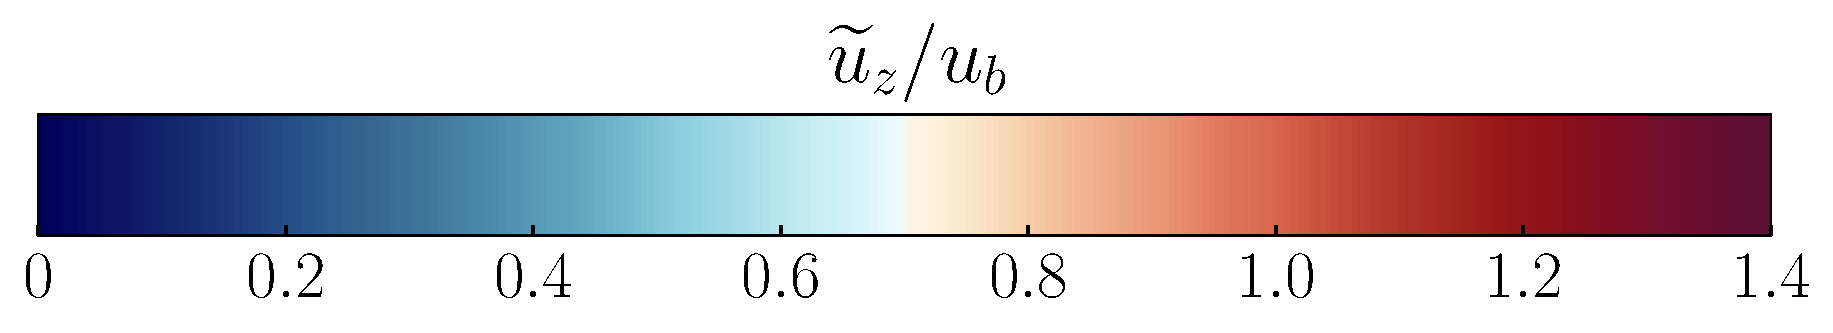
\includegraphics[width=0.5\textwidth]{Figures/uz_cmap.eps}
		\caption{
			Instantaneous axial velocity contours at $\Rey_b = 17000$
			in the cross-stream plane.
			Contour levels ranging from 0 to 1.4 are shown,
			in colour scale from blue to red. 
			The pressure side of the pipe is on the left, and the suction side is on the right
			of each sub-panel.
			Various rotation numbers are considered:
                        (a) $N = 0.0$,
                        (b) $N = 0.0078125$,
                        (c) $N = 0.015625$,
                        (d) $N = 0.0315$,
                        (e) $N = 0.0625$,
                        (f) $N = 0.125$
                        (g) $N = 0.25$,
                        (h) $N = 0.375$,
                        (i) $N = 0.5$,
			(j) $N = 1.0$,
                        (k) $N = 2.0$.
		    }
			\label{fig:urt_500} 
	\end{figure}
	\begin{figure}
		\centering
		(a) \includegraphics[width=2.cm]{Figures/cross_rotz0_roty0_T.png}  
		(b) \includegraphics[width=2.cm]{Figures/cross_rotz0_roty0.00390625_T.png}  
		(c) \includegraphics[width=2.cm]{Figures/cross_rotz0_roty0.0078125_T.png} 
		(d) \includegraphics[width=2.cm]{Figures/cross_rotz0_roty0.015625_T.png} 
		(e) \includegraphics[width=2.cm]{Figures/cross_rotz0_roty0.03125_T.png} \\ 
		(f) \includegraphics[width=2.cm]{Figures/cross_rotz0_roty0.0625_T.png} 
		(g) \includegraphics[width=2.cm]{Figures/cross_rotz0_roty0.125_T.png}  
		(h) \includegraphics[width=2.cm]{Figures/cross_rotz0_roty0.1875_T.png} 
		(i) \includegraphics[width=2.cm]{Figures/cross_rotz0_roty0.25_T.png} 
                (j) \includegraphics[width=2.cm]{Figures/cross_rotz0_roty0.5_T.png} \\
		(k) \includegraphics[width=2.cm]{Figures/cross_rotz0_roty1.0_T.png} 
		\\ 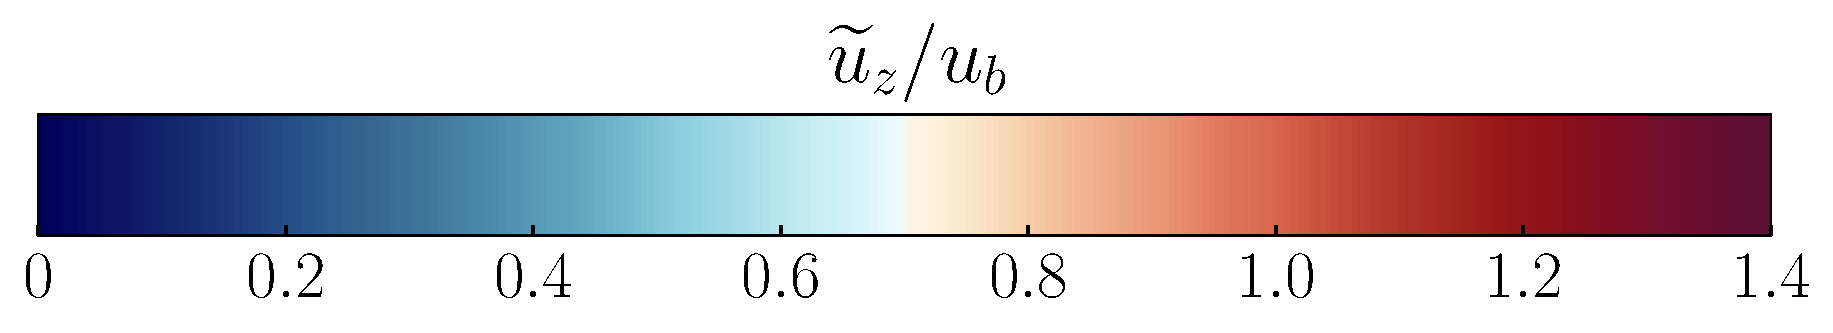
\includegraphics[width=0.5\textwidth]{Figures/uz_cmap.eps}
		\caption{
			Instantaneous temperature contours at $\Rey_b = 17000$
			in the cross-stream plane.
			Contour levels ranging from 0 to 1.4 are shown,
			in colour scale from blue to red. 
			The pressure side of the pipe is on the left, and the suction side is on the right
			of each sub-panel.
			Various rotation numbers are considered:
                        (a) $N = 0.0$,
                        (b) $N = 0.0078125$,
                        (c) $N = 0.015625$,
                        (d) $N = 0.0315$,
                        (e) $N = 0.0625$,
                        (f) $N = 0.125$
                        (g) $N = 0.25$,
                        (h) $N = 0.375$,
                        (i) $N = 0.5$,
			(j) $N = 1.0$,
                        (k) $N = 2.0$.
		}
		\label{fig:trt_500} 
	\end{figure}
	 
%	\begin{figure}
%		\centering
%		(a) \includegraphics[width=4.cm]{Figures/front_a0p005_ret3000_trim.pdf}  
%		(b) \includegraphics[width=4.cm]{Figures/front_a0p25_ret3000_trim.pdf} 
%		(c) \includegraphics[width=4.cm]{Figures/front_a8p0_ret3000_trim.pdf} \\ 
%		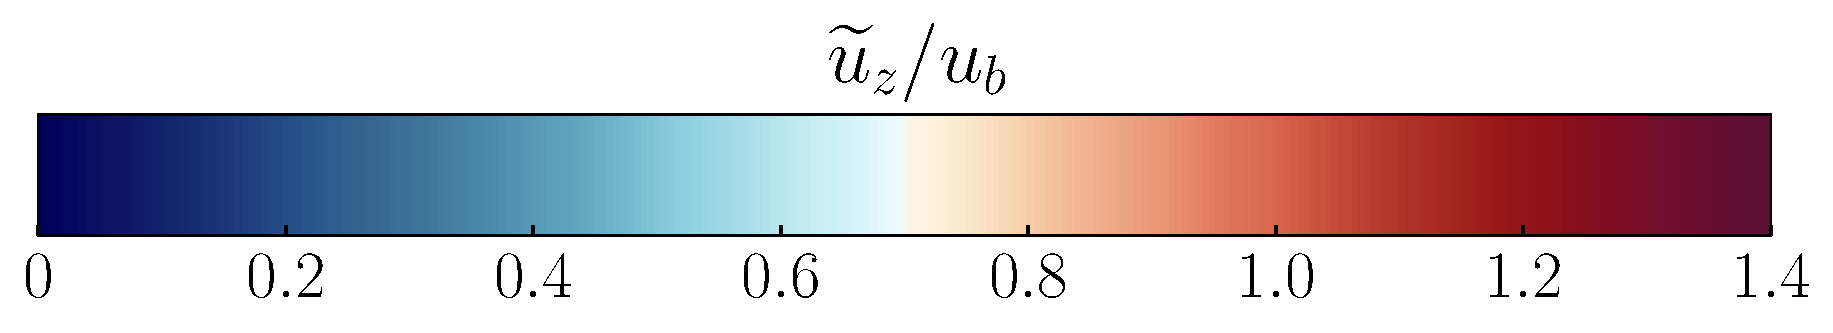
\includegraphics[width=0.5\textwidth]{Figures/uz_cmap.eps}
%		\caption{
%			Instantaneous axial velocity contours at $\Rey_b = 133000$
%			in the cross-stream plane.
%			Contour levels ranging from 0 to 1.4 are shown,
%			in colour scale from blue to red. 
%			The pressure side of the pipe is on the left, and the suction side is on the right
%			of each sub-panel.
%			Various rotation numbers are considered:
%			(a) $N = 0.01$,
%			(b) $N = 0.5$,
%			(c) $N = 16.0$.
%		    }
%			\label{fig:urt_3000} 
%	\end{figure}
	 
	\begin{figure}
		\centering
		(a) \includegraphics[width=6.cm]{Figures/unrolled_rotz0_roty0_u.png}  
                (b) \includegraphics[width=6.cm]{Figures/unrolled_rotz0_roty0.00390625_T.png} \\
		(b) \includegraphics[width=6.cm]{Figures/unrolled_rotz0_roty0.0078125_u.png}  
		(c) \includegraphics[width=6.cm]{Figures/unrolled_rotz0_roty0.015625_u.png} \\
		(d) \includegraphics[width=6.cm]{Figures/unrolled_rotz0_roty0.03125_u.png} 
                (e) \includegraphics[width=6.cm]{Figures/unrolled_rotz0_roty0.0625_u.png} \\
                (f) \includegraphics[width=6.cm]{Figures/unrolled_rotz0_roty0.125_u.png} 
                (g) \includegraphics[width=6.cm]{Figures/unrolled_rotz0_roty0.1875_u.png} \\ 
		(h) \includegraphics[width=6.cm]{Figures/unrolled_rotz0_roty0.25_u.png} 
		(i) \includegraphics[width=6.cm]{Figures/unrolled_rotz0_roty0.5_u.png} \\
                (j) \includegraphics[width=6.cm]{Figures/unrolled_rotz0_roty1.0_u.png} 
		\\ 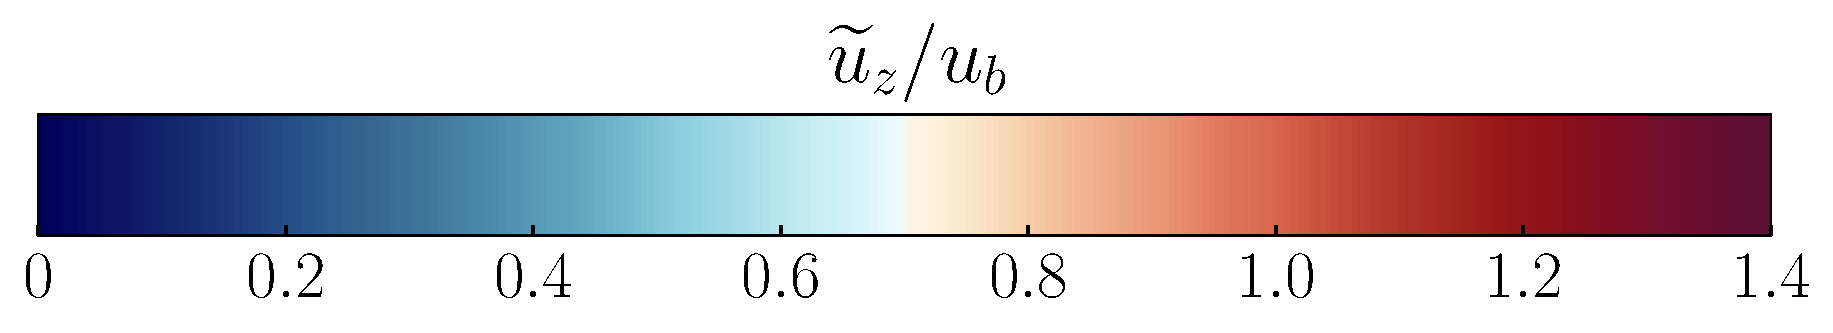
\includegraphics[width=0.5\textwidth]{Figures/uz_cmap.eps}
		\caption{
			Instantaneous axial velocity ($u_z/u_b$) contours at $\Rey_b = 17000$
			in an unrolled cylindrical shell at a distance
			$y^*=15$ from the wall (evaluated in the non-rotating case).
			Contour levels ranging from 0 to 1.4 are shown,
			in colour scale from blue to red. 
			The insets in the top-right corner of each panel report magnified views of a small portion of the shell.
			Various rotation numbers are considered:
                        (a) $N = 0.0$,
                        (b) $N = 0.0078125$,
                        (c) $N = 0.015625$,
                        (d) $N = 0.0315$,
                        (e) $N = 0.0625$,
                        (f) $N = 0.125$
                        (g) $N = 0.25$,
                        (h) $N = 0.375$,
                        (i) $N = 0.5$,
                        (j) $N = 1.0$,
                        (k) $N = 2.0$.
		}
			\label{fig:utz_500} 
	\end{figure}
	 
	\begin{figure}
		\centering
                (a) \includegraphics[width=6.cm]{Figures/unrolled_rotz0_roty0_T.png}
                (b) \includegraphics[width=6.cm]{Figures/unrolled_rotz0_roty0.00390625_T.png} \\
                (c) \includegraphics[width=6.cm]{Figures/unrolled_rotz0_roty0.0078125_T.png} 
                (d) \includegraphics[width=6.cm]{Figures/unrolled_rotz0_roty0.015625_T.png} \\
                (e) \includegraphics[width=6.cm]{Figures/unrolled_rotz0_roty0.03125_T.png} 
                (f) \includegraphics[width=6.cm]{Figures/unrolled_rotz0_roty0.0625_T.png} \\
                (f) \includegraphics[width=6.cm]{Figures/unrolled_rotz0_roty0.125_T.png} 
                (g) \includegraphics[width=6.cm]{Figures/unrolled_rotz0_roty0.1875_T.png} \\ 
                (h) \includegraphics[width=6.cm]{Figures/unrolled_rotz0_roty0.25_T.png} 
                (i) \includegraphics[width=6.cm]{Figures/unrolled_rotz0_roty0.5_T.png} \\
                jj) \includegraphics[width=6.cm]{Figures/unrolled_rotz0_roty1.0_T.png} 
		\\ \includegraphics[width=0.5\textwidth]{Figures/uz_cmap.eps}
		\caption{
			Instantaneous temperature ($t_z/t_b$) at $\Rey_b = 17000$
			in an unrolled cylindrical shell at a distance
			$y^*=15$ from the wall (evaluated in the non-rotating case).
			Contour levels ranging from 0 to 1.4 are shown,
			in colour scale from blue to red. 
			The insets in the top-right corner of each panel report magnified views of a small portion of the shell.
			Various rotation numbers are considered:
                        (a) $N = 0.0$,
                        (b) $N = 0.0078125$,
                        (c) $N = 0.015625$,
                        (d) $N = 0.0315$,
                        (e) $N = 0.0625$,
                        (f) $N = 0.125$
                        (g) $N = 0.25$,
                        (h) $N = 0.375$,
                        (i) $N = 0.5$,
                        (j) $N = 1.0$,
                        (k) $N = 2.0$.
		    }
			\label{fig:ttz_3000} 
	\end{figure}
	 
	\begin{figure}
		\centering
		(a) \includegraphics[width=2.cm]{Figures/meanfield_rotz0_roty0_u.png}  
		(b) \includegraphics[width=2.cm]{Figures/meanfield_rotz0_roty0.00390625_u.png}  
		(c) \includegraphics[width=2.cm]{Figures/meanfield_rotz0_roty0.0078125_u.png} 
		(d) \includegraphics[width=2.cm]{Figures/meanfield_rotz0_roty0.015625_u.png} 
		(e) \includegraphics[width=2.cm]{Figures/meanfield_rotz0_roty0.03125_u.png} \\ 
		(f) \includegraphics[width=2.cm]{Figures/meanfield_rotz0_roty0.0625_u.png} 
		(g) \includegraphics[width=2.cm]{Figures/meanfield_rotz0_roty0.125_u.png}  
		(h) \includegraphics[width=2.cm]{Figures/meanfield_rotz0_roty0.1875_u.png} 
		(i) \includegraphics[width=2.cm]{Figures/meanfield_rotz0_roty0.25_u.png} 
                (j) \includegraphics[width=2.cm]{Figures/meanfield_rotz0_roty0.5_u.png} \\
		(k) \includegraphics[width=2.cm]{Figures/meanfield_rotz0_roty1.0_u.png} 
		\\ \includegraphics[width=0.5\textwidth]{Figures/uzmean_cmap.eps}
		\caption{
			Mean axial velocity contours with 
			superposed cross-flow streamlines, at $\Rey_b = 17000$.
			Twenty-four contour levels ranging from 0 to 1.4 are shown,
			in colour scale from blue to red. 
			The pressure side of the pipe is on the left, and the suction side is on the right
			of each sub-panel.
			Various rotation numbers are considered:
                        (a) $N = 0.0$,
                        (b) $N = 0.0078125$,
                        (c) $N = 0.015625$,
                        (d) $N = 0.0315$,
                        (e) $N = 0.0625$,
                        (f) $N = 0.125$
                        (g) $N = 0.25$,
                        (h) $N = 0.375$,
                        (i) $N = 0.5$,
			(j) $N = 1.0$,
                        (k) $N = 2.0$.	
		    }
			\label{fig:Urt_500} 
	\end{figure}

	\begin{figure}
                \centering
                (a) \includegraphics[width=2.cm]{Figures/meanfield_rotz0_roty0_T.png}
                (b) \includegraphics[width=2.cm]{Figures/meanfield_rotz0_roty0.00390625_T.png}
                (c) \includegraphics[width=2.cm]{Figures/meanfield_rotz0_roty0.0078125_T.png}
                (d) \includegraphics[width=2.cm]{Figures/meanfield_rotz0_roty0.015625_T.png}
                (e) \includegraphics[width=2.cm]{Figures/meanfield_rotz0_roty0.03125_T.png} \\
                (f) \includegraphics[width=2.cm]{Figures/meanfield_rotz0_roty0.0625_T.png}
                (g) \includegraphics[width=2.cm]{Figures/meanfield_rotz0_roty0.125_T.png}
                (h) \includegraphics[width=2.cm]{Figures/meanfield_rotz0_roty0.1875_T.png}
                (i) \includegraphics[width=2.cm]{Figures/meanfield_rotz0_roty0.25_T.png}
                (j) \includegraphics[width=2.cm]{Figures/meanfield_rotz0_roty0.5_T.png}
                (k) \includegraphics[width=2.cm]{Figures/meanfield_rotz0_roty1.0_T.png}
                \\ \includegraphics[width=0.5\textwidth]{Figures/uzmean_cmap.eps}
                \caption{
                        Mean temperature contours with
                        superposed cross-flow streamlines, at $\Rey_b = 17000$.
                        Twenty-four contour levels ranging from 0 to 1.4 are shown,
                        in colour scale from blue to red.
                        The pressure side of the pipe is on the left, and the suction side is on the right
                        of each sub-panel.
                        Various rotation numbers are considered:
                        (a) $N = 0.0$,
                        (b) $N = 0.0078125$,
                        (c) $N = 0.015625$,
                        (d) $N = 0.0315$,
                        (e) $N = 0.0625$,
                        (f) $N = 0.125$
			(g) $N = 0.25$,
                        (h) $N = 0.375$,
                        (i) $N = 0.5$,
			(j) $N = 1.0$,
                        (k) $N = 2.0$.
                    }
                        \label{fig:Trt_500}
        \end{figure}


%	\begin{figure}
%		\centering
%		(a)
%		\includegraphics[width=3.cm]{Figures/meanupsi_RETAU3000_ROTATING_Y_A0p005_CORIOLIS.eps}   
%		(b)
%		\includegraphics[width=3.cm]{Figures/meanupsi_RETAU3000_ROTATING_Y_A0p25_CORIOLIS.eps} 
%		(c)
%		\includegraphics[width=3.cm]{Figures/meanupsi_RETAU3000_ROTATING_Y_A8p0_CORIOLIS.eps}  
%    		\\ \includegraphics[width=0.5\textwidth]{Figures/uzmean_cmap.eps}
%		\caption{
%			Mean axial velocity contours with 
%			superposed cross-flow streamlines, at $\Rey_b = 133000$.
%			Twenty-four contour levels ranging from 0 to 1.4 are shown,
%			in colour scale from blue to red. 
%			The pressure side of the pipe is on the left, and the suction side is on the right
%			of each sub-panel.
%			Various rotation numbers are considered:
%			(a) $N = 0.01$,
%			(b) $N = 0.5$,
%			(c) $N = 16.0$.
%		    }
%			\label{fig:Urt_3000} 
%	\end{figure}
	
%	\begin{figure}
%		\centering
%		(a) \includegraphics[width=5.25cm]{Figures/cf_azimuth_500.eps}   
%		(b) \includegraphics[width=5.25cm]{Figures/cf_azimuth_norm_500.eps} \\
%		(c) \includegraphics[width=5.25cm]{Figures/cf_azimuth_3000.eps}   
%		(d) \includegraphics[width=5.25cm]{Figures/cf_azimuth_norm_3000.eps} \\
%		\caption{
%			Polar distribution of the \textcolor{blue}{local streamwise wall shear stress} ($\tau_w$),
%	                normalised by either the reference dynamic pressure $\rho u_b ^2$ (a, c),
%                 	or the mean wall shear stress $\tau_w^*$ (b, d), at 
%			$\Rey_b=17000$ (a, b), and $\Rey_b=133000$ (c, d).
%			The color codes correspond to different values of $N$, 
%			as given in table~\ref{tab:runs},
%			gray denoting cases without rotation.
%			The dashed blue line in panels (a, c)
%			denotes the predictive formula given in equation~\eqref{eq:fric_polar}.
%			}
%			\label{fig:Cf_polar} 
%	\end{figure}

	\begin{figure}
		\centering
		(a) \includegraphics[width=4cm]{Figures/prof_uzub_rotz0_roty0.00390625.eps}
                (b) \includegraphics[width=4cm]{Figures/prof_uzub_rotz0_roty0.0078125.eps} \\
                (c) \includegraphics[width=4cm]{Figures/prof_uzub_rotz0_roty0.015625.eps}
                (d) \includegraphics[width=4cm]{Figures/prof_uzub_rotz0_roty0.03125.eps} \\
                (e) \includegraphics[width=4cm]{Figures/prof_uzub_rotz0_roty0.0625.eps} 
                (f) \includegraphics[width=4cm]{Figures/prof_uzub_rotz0_roty0.125.eps} \\
                (g) \includegraphics[width=4cm]{Figures/prof_uzub_rotz0_roty0.1875.eps}
                (h) \includegraphics[width=4cm]{Figures/prof_uzub_rotz0_roty0.25.eps} \\
                (i) \includegraphics[width=4cm]{Figures/prof_uzub_rotz0_roty0.5.eps}
		(j) \includegraphics[width=4cm]{Figures/prof_uzub_rotz0_roty1.0.eps} \\ 
    		\includegraphics[width=0.5\textwidth]{Figures/theta_cmap_half.eps}
     		\caption{
    		Radial profiles of 
    		outer-scaled axial velocity 
    		at various azimuthal positions, 
		for flow cases at $\Rey_b=17000$.
		Only the interval $\theta = [0^{\circ},90^{\circ}]$ is shown, at stations
		spaced $7.5^\circ$ apart, with negative values of $r$ signifying profiles
		taken at $\theta + 180^{\circ}$.
                (a) $N = 0.0078125$,
                (b) $N = 0.015625$,
                (c) $N = 0.0315$,
                (d) $N = 0.0625$,
                (e) $N = 0.125$
                (f) $N = 0.25$,
                (g) $N = 0.375$,
                (h) $N = 0.5$,
                (i) $N = 1.0$,
                (j) $N = 2.0$.
		The black solid line denotes the mean axial velocity profile in the
    		non-rotating case.
    	}
	\label{fig:uprof}
	\end{figure}

        \begin{figure}
                \centering
		(a) \includegraphics[width=4cm]{Figures/prof_tttb_rotz0_roty0.00390625.eps} 
		(b) \includegraphics[width=4cm]{Figures/prof_tttb_rotz0_roty0.0078125.eps} \\
		(c) \includegraphics[width=4cm]{Figures/prof_tttb_rotz0_roty0.015625.eps}
		(d) \includegraphics[width=4cm]{Figures/prof_tttb_rotz0_roty0.03125.eps} \\
                (e) \includegraphics[width=4cm]{Figures/prof_tttb_rotz0_roty0.0625.eps} 
                (f) \includegraphics[width=4cm]{Figures/prof_tttb_rotz0_roty0.125.eps} \\
                (g) \includegraphics[width=4cm]{Figures/prof_tttb_rotz0_roty0.1875.eps}
                (h) \includegraphics[width=4cm]{Figures/prof_tttb_rotz0_roty0.25.eps} \\
                (i) \includegraphics[width=4cm]{Figures/prof_tttb_rotz0_roty0.5.eps}
                (j) \includegraphics[width=4cm]{Figures/prof_tttb_rotz0_roty1.0.eps} \\
                \includegraphics[width=0.5\textwidth]{Figures/theta_cmap_half.eps}
                \caption{
                Radial profiles of
                outer-scaled temperature
                at various azimuthal positions,
                for flow cases at $\Rey_b=17000$.
                Only the interval $\theta = [0^{\circ},90^{\circ}]$ is shown, at stations
                spaced $7.5^\circ$ apart, with negative values of $r$ signifying profiles
                taken at $\theta + 180^{\circ}$.
                (a) $N = 0.0078125$,
                (b) $N = 0.015625$,
                (c) $N = 0.0315$,
                (d) $N = 0.0625$,
                (e) $N = 0.125$
                (f) $N = 0.25$,
                (g) $N = 0.375$,
                (h) $N = 0.5$,
                (i) $N = 1.0$,
                (j) $N = 2.0$.
                The black solid line denotes the mean axial velocity profile in the
                non-rotating case.
        }
        \label{fig:tprof}
        \end{figure}

	 
        \begin{figure}
    	\centering
		(a) \includegraphics[width=4cm]{Figures/prof_uzplus_rotz0_roty0.00390625.eps}
                (b) \includegraphics[width=4cm]{Figures/prof_uzplus_rotz0_roty0.0078125.eps} \\
                (c) \includegraphics[width=4cm]{Figures/prof_uzplus_rotz0_roty0.015625.eps}
                (d) \includegraphics[width=4cm]{Figures/prof_uzplus_rotz0_roty0.03125.eps} \\
                (e) \includegraphics[width=4cm]{Figures/prof_uzplus_rotz0_roty0.0625.eps}
                (f) \includegraphics[width=4cm]{Figures/prof_uzplus_rotz0_roty0.125.eps} \\
                (g) \includegraphics[width=4cm]{Figures/prof_uzplus_rotz0_roty0.1875.eps}
                (h) \includegraphics[width=4cm]{Figures/prof_uzplus_rotz0_roty0.25.eps} \\
                (i) \includegraphics[width=4cm]{Figures/prof_uzplus_rotz0_roty0.5.eps}
                (j) \includegraphics[width=4cm]{Figures/prof_uzplus_rotz0_roty1.0.eps} \\
	    	\includegraphics[width=0.5\textwidth]{Figures/theta_cmap.eps}
    	\caption{
    		Wall-normal profiles of 
    		inner-scaled axial velocity,
    		at various azimuthal positions spaced 
		$7.5^\circ$ apart,
		for flow cases at $\Rey_b=17000$.
		Only the interval $\theta = [0^{\circ},180^{\circ}]$ is shown.
    	        (a) $N = 0.0078125$,
                (b) $N = 0.015625$,
                (c) $N = 0.0315$,
                (d) $N = 0.0625$,
                (e) $N = 0.125$
                (f) $N = 0.25$,
                (g) $N = 0.375$,
                (h) $N = 0.5$,
                (i) $N = 1.0$,
                (j) $N = 2.0$.	
    		The black solid line denotes the mean axial velocity profile in the
    		non-rotating case.
    		The dashed gray lines depict the compound law-of-the wall
    		$U^+=y^+$, $U^+=\log y^+/0.387 + 4.53$.
    	}
		\label{fig:uplus}
	\end{figure}

        \begin{figure}
        \centering
                (a) \includegraphics[width=4cm]{Figures/prof_ttplus_rotz0_roty0.00390625.eps}
                (b) \includegraphics[width=4cm]{Figures/prof_ttplus_rotz0_roty0.0078125.eps} \\
                (c) \includegraphics[width=4cm]{Figures/prof_ttplus_rotz0_roty0.015625.eps}
                (d) \includegraphics[width=4cm]{Figures/prof_ttplus_rotz0_roty0.03125.eps} \\
                (e) \includegraphics[width=4cm]{Figures/prof_ttplus_rotz0_roty0.0625.eps}
                (f) \includegraphics[width=4cm]{Figures/prof_ttplus_rotz0_roty0.125.eps} \\
                (g) \includegraphics[width=4cm]{Figures/prof_ttplus_rotz0_roty0.1875.eps}
                (h) \includegraphics[width=4cm]{Figures/prof_ttplus_rotz0_roty0.25.eps} \\
                (i) \includegraphics[width=4cm]{Figures/prof_ttplus_rotz0_roty0.5.eps}
                (j) \includegraphics[width=4cm]{Figures/prof_ttplus_rotz0_roty1.0.eps} \\
                \includegraphics[width=0.5\textwidth]{Figures/theta_cmap.eps}
        \caption{
                Wall-normal profiles of
                inner-scaled temperature,
                at various azimuthal positions spaced
                $7.5^\circ$ apart,
                for flow cases at $\Rey_b=17000$.
                Only the interval $\theta = [0^{\circ},180^{\circ}]$ is shown.
                (a) $N = 0.0078125$,
                (b) $N = 0.015625$,
                (c) $N = 0.0315$,
                (d) $N = 0.0625$,
                (e) $N = 0.125$
                (f) $N = 0.25$,
                (g) $N = 0.375$,
                (h) $N = 0.5$,
                (i) $N = 1.0$,
                (j) $N = 2.0$.
                The black solid line denotes the mean temperature profile in the
                non-rotating case.
                The dashed gray lines depict the compound law-of-the wall
		$\theta^{+}=y^+$, $\theta^{+}=\log y^+/0.387 + 4.53$.
        }
                \label{fig:tplus}
        \end{figure}

        \begin{figure}
        \centering
                (a) \includegraphics[width=4cm]{Figures/prof_uzstar_rotz0_roty0.00390625.eps}
                (b) \includegraphics[width=4cm]{Figures/prof_uzstar_rotz0_roty0.0078125.eps} \\
                (c) \includegraphics[width=4cm]{Figures/prof_uzstar_rotz0_roty0.015625.eps}
                (d) \includegraphics[width=4cm]{Figures/prof_uzstar_rotz0_roty0.03125.eps} \\
                (e) \includegraphics[width=4cm]{Figures/prof_uzstar_rotz0_roty0.0625.eps}
                (f) \includegraphics[width=4cm]{Figures/prof_uzstar_rotz0_roty0.125.eps} \\
                (g) \includegraphics[width=4cm]{Figures/prof_uzstar_rotz0_roty0.1875.eps}
                (h) \includegraphics[width=4cm]{Figures/prof_uzstar_rotz0_roty0.25.eps} \\
                (i) \includegraphics[width=4cm]{Figures/prof_uzstar_rotz0_roty0.5.eps}
                (j) \includegraphics[width=4cm]{Figures/prof_uzstar_rotz0_roty1.0.eps} \\
                \includegraphics[width=0.5\textwidth]{Figures/theta_cmap.eps}
        \caption{
                Wall-normal profiles of
                outer-scaled axial velocity,
                at various azimuthal positions spaced
                $7.5^\circ$ apart,
                for flow cases at $\Rey_b=17000$.
                Only the interval $\theta = [0^{\circ},180^{\circ}]$ is shown.
                (a) $N = 0.0078125$,
                (b) $N = 0.015625$,
                (c) $N = 0.0315$,
                (d) $N = 0.0625$,
                (e) $N = 0.125$
                (f) $N = 0.25$,
                (g) $N = 0.375$,
                (h) $N = 0.5$,
                (i) $N = 1.0$,
                (j) $N = 2.0$.
                The black solid line denotes the mean axial velocity profile in the
                non-rotating case.
                The dashed gray lines depict the compound law-of-the wall
                $U^*=y^*$, $U^*=\log y^*/0.387 + 4.53$.
        }
                \label{fig:ustar}
        \end{figure}

	\begin{figure}
        \centering
                (a) \includegraphics[width=4cm]{Figures/prof_ttstar_rotz0_roty0.00390625.eps}
                (b) \includegraphics[width=4cm]{Figures/prof_ttstar_rotz0_roty0.0078125.eps} \\
                (c) \includegraphics[width=4cm]{Figures/prof_ttstar_rotz0_roty0.015625.eps}
                (d) \includegraphics[width=4cm]{Figures/prof_ttstar_rotz0_roty0.03125.eps} \\
                (e) \includegraphics[width=4cm]{Figures/prof_ttstar_rotz0_roty0.0625.eps}
                (f) \includegraphics[width=4cm]{Figures/prof_ttstar_rotz0_roty0.125.eps} \\
                (g) \includegraphics[width=4cm]{Figures/prof_ttstar_rotz0_roty0.1875.eps}
                (h) \includegraphics[width=4cm]{Figures/prof_ttstar_rotz0_roty0.25.eps} \\
                (i) \includegraphics[width=4cm]{Figures/prof_ttstar_rotz0_roty0.5.eps}
                (j) \includegraphics[width=4cm]{Figures/prof_ttstar_rotz0_roty1.0.eps} \\
                \includegraphics[width=0.5\textwidth]{Figures/theta_cmap.eps}
        \caption{
                Wall-normal profiles of
                outer-scaled temperature,
                at various azimuthal positions spaced
                $7.5^\circ$ apart,
                for flow cases at $\Rey_b=17000$.
                Only the interval $\theta = [0^{\circ},180^{\circ}]$ is shown.
                (a) $N = 0.0078125$,
                (b) $N = 0.015625$,
                (c) $N = 0.0315$,
                (d) $N = 0.0625$,
                (e) $N = 0.125$
                (f) $N = 0.25$,
                (g) $N = 0.375$,
                (h) $N = 0.5$,
                (i) $N = 1.0$,
                (j) $N = 2.0$.
                The black solid line denotes the mean temperature profile in the
                non-rotating case.
                The dashed gray lines depict the compound law-of-the wall
		$\theta^{*}=y^*$, $\theta^{*}=\log y^*/0.387 + 4.53$.
        }
                \label{fig:tstar}
        \end{figure}

       \begin{figure}
       \centering
 	       (a) \includegraphics[width=4cm]{Figures/prof_tkeouter_rotz0_roty0.00390625.eps}
               (b) \includegraphics[width=4cm]{Figures/prof_tkeouter_rotz0_roty0.0078125.eps} \\
               (c) \includegraphics[width=4cm]{Figures/prof_tkeouter_rotz0_roty0.015625.eps}
               (d) \includegraphics[width=4cm]{Figures/prof_tkeouter_rotz0_roty0.03125.eps} \\
               (e) \includegraphics[width=4cm]{Figures/prof_tkeouter_rotz0_roty0.0625.eps}
               (f) \includegraphics[width=4cm]{Figures/prof_tkeouter_rotz0_roty0.125.eps} \\
               (g) \includegraphics[width=4cm]{Figures/prof_tkeouter_rotz0_roty0.1875.eps}
               (h) \includegraphics[width=4cm]{Figures/prof_tkeouter_rotz0_roty0.25.eps} \\
               (i) \includegraphics[width=4cm]{Figures/prof_tkeouter_rotz0_roty0.5.eps}
               (j) \includegraphics[width=4cm]{Figures/prof_tkeouter_rotz0_roty1.0.eps} \\
               \includegraphics[width=0.5\textwidth]{Figures/theta_cmap_half.eps} \\
       \caption{
               Radial profiles of 
               outer-scaled turbulence kinetic energy
               at various azimuthal positions, 
               for flow cases at $\Rey_b=17000$.
               Only the interval $\theta = [0^{\circ},90^{\circ}]$ is shown, at stations
               spaced $7.5^\circ$ apart, with negative values of $r$ signifying profiles
               taken at $\theta + 180^{\circ}$.
               (a) $N = 0.0078125$,
               (b) $N = 0.015625$,
               (c) $N = 0.0315$,
               (d) $N = 0.0625$,
               (e) $N = 0.125$
               (f) $N = 0.25$,
               (g) $N = 0.375$,
               (h) $N = 0.5$,
               (i) $N = 1.0$,
               (j) $N = 2.0$. 
               The black solid line denotes the mean turbulence kinetic energy profile in the
               non-rotating case.
               }
               \label{fig:tke}
       \end{figure}
       
       \begin{figure}
       \centering
               (a) \includegraphics[width=4cm]{Figures/prof_rssouter_rotz0_roty0.00390625.eps}
               (b) \includegraphics[width=4cm]{Figures/prof_rssouter_rotz0_roty0.0078125.eps} \\
               (c) \includegraphics[width=4cm]{Figures/prof_rssouter_rotz0_roty0.015625.eps}
               (d) \includegraphics[width=4cm]{Figures/prof_rssouter_rotz0_roty0.03125.eps} \\
               (e) \includegraphics[width=4cm]{Figures/prof_rssouter_rotz0_roty0.0625.eps}
               (f) \includegraphics[width=4cm]{Figures/prof_rssouter_rotz0_roty0.125.eps} \\
               (g) \includegraphics[width=4cm]{Figures/prof_rssouter_rotz0_roty0.1875.eps}
               (h) \includegraphics[width=4cm]{Figures/prof_rssouter_rotz0_roty0.25.eps} \\
               (i) \includegraphics[width=4cm]{Figures/prof_rssouter_rotz0_roty0.5.eps}
               (j) \includegraphics[width=4cm]{Figures/prof_rssouter_rotz0_roty1.0.eps} \\
               \includegraphics[width=0.5\textwidth]{Figures/theta_cmap_half.eps} \\
       \caption{
               Radial profiles of
               outer-scaled Reynolds shear stress
               at various azimuthal positions,
               for flow cases at $\Rey_b=17000$.
               Only the interval $\theta = [0^{\circ},90^{\circ}]$ is shown, at stations
               spaced $7.5^\circ$ apart, with negative values of $r$ signifying profiles
               taken at $\theta + 180^{\circ}$.
               (a) $N = 0.0078125$,
               (b) $N = 0.015625$,
               (c) $N = 0.0315$,
               (d) $N = 0.0625$,
               (e) $N = 0.125$
               (f) $N = 0.25$,
               (g) $N = 0.375$,
               (h) $N = 0.5$,
               (i) $N = 1.0$,
               (j) $N = 2.0$.
	       The black solid line denotes the Reynolds shear stress profile in the
               non-rotating case.
               }
               \label{fig:rss}
       \end{figure}


%	\begin{figure}
%		\centering
%		(a)
%		\includegraphics[width=5.25cm]{Figures/scaling_uzplus_500.eps}
%		(b)
%		\includegraphics[width=5.25cm]{Figures/scaling_uzplus_3000.eps}
%		\\
%		\caption{
%			Inner-scaled wall-normal mean velocity profiles at $\theta = 180^\circ$ (pressure side).
%			Solid lines refer to DNS data and dashed lines to equation~\eqref{eq:yang}, for flow
%			cases at $\Rey_b = 17000$ (a) and cases at $\Rey_b = 133000$ (b).
%			Color codes are as in table~\ref{tab:runs}.
%		    }
%		\label{fig:yang}
%	\end{figure}
%
%
%	\begin{figure}
%    	\centering
%		\begin{tabular}{llll}
%			\includegraphics[width=3.0cm]{Figures/tke_RETAU500_ROTATING_Y_A0p015625_CORIOLIS.eps}  &
%			\includegraphics[width=3.0cm]{Figures/tke_RETAU500_ROTATING_Y_A0p25_CORIOLIS.eps}  &
%			\includegraphics[width=3.0cm]{Figures/tke_RETAU500_ROTATING_Y_A1p0_CORIOLIS.eps}  &
%		\includegraphics[width=3.0cm]{Figures/tke_RETAU500_ROTATING_Y_A4p0_CORIOLIS.eps} \\
%			(a) & (b) & (c) & (d) \\
%			\includegraphics[width=3.0cm]{Figures/tke_RETAU3000_ROTATING_Y_A0p05_CORIOLIS.eps}  &
%			\includegraphics[width=3.0cm]{Figures/tke_RETAU3000_ROTATING_Y_A0p25_CORIOLIS.eps}  &
%			\includegraphics[width=3.0cm]{Figures/tke_RETAU3000_ROTATING_Y_A1p0_CORIOLIS.eps}  &
%		\includegraphics[width=3.0cm]{Figures/tke_RETAU3000_ROTATING_Y_A8p0_CORIOLIS.eps} \\
%			(e) & (f) & (g) & (h) \\
%		\end{tabular}
%		\\
%		\includegraphics[width=0.5\textwidth]{Figures/theta_cmap_half.eps} \\
%    	\caption{
%    		Radial profiles of 
%    		outer-scaled turbulence kinetic energy
%    		at various azimuthal positions, 
%		for flow cases at $\Rey_b=17000$ (a-d), and $\Rey_b=133000$ (e-h).
%		Only the interval $\theta = [0^{\circ},90^{\circ}]$ is shown, at stations
%		spaced $7.5^\circ$ apart, with negative values of $r$ signifying profiles
%		taken at $\theta + 180^{\circ}$.
%    		(a) $N = 0.03125$,
%    		(b) $N = 0.5$,
%    		(c) $N = 2.0$,
%    		(d) $N = 8.0$.
%		(e) $N = 0.1$,
%		(f) $N = 0.5$,
%		(g) $N = 2.0$,
%		(h) $N = 16.0$.
%    		The black solid line denotes the mean turbulence kinetic energy profile in the
%    		non-rotating case.
%		}
%		\label{fig:tke}
%	\end{figure}
%	 
	\begin{figure}
    	\centering
		\begin{tabular}{lll}
		\includegraphics[width=4.cm]{Figures/ekman_profsy_roty_500_u.eps} &
		\includegraphics[width=4.cm]{Figures/ekman_angles_roty_500_u.eps} &
		\includegraphics[width=4.cm]{Figures/ekman_spiral_roty_500_u.eps} \\
		(a) & (b) & (c) \\	
		\end{tabular}
    	\caption{
    		Profiles of 
		mean axial ($U_z$) and azimuthal ($U_\theta$) velocity
		(a), wall-parallel flow angle $\varphi = \tan^{-1} (U_{\theta}/U_z)$ (b) 
		and hodograph diagram (c) 
		at the polar coordinate $\theta = \pi/2$ (north pole of the pipe).
		Data are shown for $\Rey_b=17000$, at various rotation numbers:
    		(a) $N = 0.0078125$,
                (b) $N = 0.015625$,
                (c) $N = 0.0315$,
                (d) $N = 0.0625$,
                (e) $N = 0.125$
                (f) $N = 0.25$,
                (g) $N = 0.375$,
                (h) $N = 0.5$,
                (i) $N = 1.0$,
                (j) $N = 2.0$.
		see table~\ref{tab:runs} for the color codes.
    		The velocity profiles are scaled by the 
    		mean centreline axial velocity $U_{0}$.
    		The black circles denote the analytical solution 
		for a laminar Ekman layer~\citep{greenspan1968}.
    	}
		\label{fig:Ekman_500}
	\end{figure}

        \begin{figure}
        \centering
                \begin{tabular}{ll}
                \includegraphics[width=5.cm]{Figures/ekman_profsyr_roty_500_T.eps} &
                \includegraphics[width=5.cm]{Figures/ekman_profsyd_roty_500_T.eps} \\ 
			(a) & (b) \\
                \end{tabular}
        \caption{
                Profiles of
		the temperature $\Theta$ plotted at the poles of the pipe
                as a function of the radial coordinate normalised by the pipe radius (a) and the wall normal coordinate
                normalised by the local Ekman layer thickness (b).
                Data are shown for $\Rey_b=17000$, at various rotation numbers:
                (a) $N = 0.0078125$,
                (b) $N = 0.015625$,
                (c) $N = 0.0315$,
                (d) $N = 0.0625$,
                (e) $N = 0.125$
                (f) $N = 0.25$,
                (g) $N = 0.375$,
                (h) $N = 0.5$,
                (i) $N = 1.0$,
                (j) $N = 2.0$.
		see table~\ref{tab:runs} for the color codes.
                The temperature profiles are scaled by the
                temperature at the center of the pipe $T_{CL}$.
        }
                \label{fig:Ekman_T_500}
        \end{figure}

        \begin{figure}
        \centering
                \begin{tabular}{ll}
                \includegraphics[width=5.cm]{Figures/ekman_profsyr_roty_500_T_alternative.eps} &
		\includegraphics[width=5.cm]{Figures/ekman_profsyd_roty_500_T_alternative.eps} \\
                (a) & (b) \\
                \end{tabular}
        \caption{
                Profiles of
		the temperature $\Theta$ plotted at the poles of the pipe 
		as a function of the radial coordinate normalised by the pipe radius (a) and the wall normal coordinate 
		normalised by the local Ekman layer thickness (b).  
                Data are shown for $\Rey_b=17000$, at various rotation numbers:
                (a) $N = 0.0078125$,
                (b) $N = 0.015625$,
                (c) $N = 0.0315$,
                (d) $N = 0.0625$,
                (e) $N = 0.125$
                (f) $N = 0.25$,
                (g) $N = 0.375$,
                (h) $N = 0.5$,
                (i) $N = 1.0$,
                (j) $N = 2.0$.
                see table~\ref{tab:runs} for the color codes.
                The temperature profiles are scaled by the
		temperature taken at the edge of the Ekman layer $T_{6\Delta}$.
        }
                \label{fig:Ekman_T_6delta_500}
        \end{figure}

	\begin{figure}
                \centering
                \begin{tabular}{lll}
		\includegraphics[width=4cm]{Figures/ch_azimuth_global_500.eps} &
		\includegraphics[width=4cm]{Figures/ch_azimuth_local_500.eps} &
                \includegraphics[width=4cm]{Figures/sra_azimuth_local_500.eps} \\
		(a) & (b) & (c) \\
                \end{tabular}
                \caption{
			Polar distribution of the ratio of the local Stanton number and the global Stanton number (a), 
			polar distribution of the local Stanton number (b)  
			and polar distribution of the local Strong Reynolds Analogy factor (c), at $\Rey_b=17000$.
                        The color codes correspond to different values of $N$,
                        as given in table~\ref{tab:runs},
                        black denoting cases without rotation.
                        }
                        \label{fig:Ch__azimuth_polar}
        \end{figure}

	\begin{figure}
                \centering
                (a) \includegraphics[width=5.25cm]{Figures//sra_global_500.eps}
                (b) \includegraphics[width=5.25cm]{Figures//ch_cf_500.eps} \\
                \caption{
			On the left the global Strong Reynolds Analogy factor as function of the rotation number $N$ (a) 
			and on the right the global Stanton number and friction coefficient as function of the rotation number (b).
                        }
                        \label{fig:Ch_Cf}
        \end{figure}


%	\begin{figure}
%		\centering
%		\begin{tabular}{lll}
%		\includegraphics[width=4.cm]{Figures/ekman_uz_utheta_3000.eps} &
%		\includegraphics[width=4.cm]{Figures/ekman_angle_3000.eps} &
%		\includegraphics[width=4.cm]{Figures/ekman_spiral_3000.eps} \\
%		(a) & (b) & (c) \\
%		\end{tabular}
%    	\caption{
%    		Profiles of 
%		mean axial ($U_z$) and azimuthal ($U_\theta$) velocity
%		(a), wall-parallel flow angle $\varphi = \tan^{-1} (U_{\theta}/U_z)$ (b) 
%		and hodograph diagram (c) 
%		at the polar coordinate $\theta = \pi/2$ (north pole of the pipe).
%		Data are shown for $\Rey_b=133000$, at various rotation numbers:
%			$N = 0.1$,
%			$N = 0.5$,
%			$N = 2.0$,
%			$N = 16.0$,
%		see table~\ref{tab:runs} for the color codes.
%    		The velocity profiles are scaled by the 
%    		mean centreline axial velocity $U_{0}$.
%    		The black circles denote the analytical solution 
%		for a laminar Ekman layer~\citep{greenspan1968}.
%		}
%		\label{fig:Ekman_3000}
%	\end{figure}
%	 
%	\section{Friction} \label{sec:friction}
%
%	\begin{figure}
%		\centering
%		\begin{tabular}{ll}
%		\includegraphics[width=5.0cm]{Figures/scatter_500.eps} &
%		\includegraphics[width=5.0cm]{Figures/scatter_3000.eps} \\
%		(a) & (b)
%		\end{tabular}
%		\caption{
%		Scatter plots of mean axial velocity as a function of the horizontal coordinate,
%	        for $\Rey_b=17000, N = 8$ (a) and $\Rey_b=133000, N = 16$ (b), in blue.
%	        Only points at wall distance greater than five
%	        Ekman layer thicknesses are shown.
%		The black dashed lines denote the velocity profile given in equation~\eqref{eq:uzfit}.
%	}
%	        \label{fig:scatter}
%	\end{figure}
%
%	\begin{figure}
%		\centering
%		(a) \includegraphics[width=5.0cm]{Figures/ekman_theta_500.eps} 
%	        (b) \includegraphics[width=5.0cm]{Figures/ekman_theta_3000.eps} \\
%		\includegraphics[width=0.5\textwidth]{Figures/theta_cmap.eps}
%		\caption{Mean axial velocity profiles scaled by the local geostrophic velocity ($U_g$),
%		as a function of wall distance normalised by the local Ekman layer thickness,
%		$\Delta = (\nu/(\Omega \sin \theta))^{1/2}$,
%		at $\Rey_b=17000$, $N=8$ (a), and $\Rey_b=133000$, $N=16$ (b).
%		Profiles along the pipe perimeter are shown in intervals of $7.5^{\circ}$, 
%		with exception of $\theta=0^{\circ}$, $\theta=180^{\circ}$.
%		}
%		\label{fig:Uznorm} 
%	\end{figure}
%
%	\begin{figure}
%		\centering
%		\begin{tabular}{ll}
%		\includegraphics[width=6.0cm]{Figures/lambda_rotating_a.eps} &
%		\includegraphics[width=6.0cm]{Figures/lambda_rotating_b.eps} \\
%		(a) & (b) \\
%		\end{tabular}
%		\caption{
%		    Distribution of friction factor as a function of $(N/\Rey_b)^{1/2}$,
%		    for DNS data at $\Rey_b=17000$ ($\bm{+}$), $\Rey_b=44000$ ($\bm{*}$),
%		    $\Rey_b=82500$ ($\bigstar$), $\Rey_b=133000$ ($\blacksquare$).
%		    In panel (a) the solid line denotes the asymptotic prediction for the rapid-rotation regime~\eqref{eq:lambda_as}.
%		    Lines in (b) denote prediction of the interpolation formula~\eqref{eq:lambda_int} 
%		    at $\Rey_b=17000$ (blue), $\Rey_b=44000$ (red),
%                    $\Rey_b=82500$ (orange), $\Rey_b=133000$ (purple).}
%			\label{fig:lambda}
%	\end{figure}
%
%	 
%	\begin{figure}
%		\centering
%		\begin{tabular}{ll}
%		\includegraphics[width=6.0cm]{Figures/kt_lam_ito_a.eps} &
%		\includegraphics[width=6.0cm]{Figures/kt_lam_ito_b.eps} \\
%		(a) & (b) \\
%		\end{tabular}
%		\caption{
%		    Distribution of friction factor (normalised by the non-rotating case value) as a
%		    function of the parameter $K_t = \Rey_b N^2/4$~\citep{ito71},
%		    for DNS data at $\Rey_b=17000$ ($\bm{+}$), $\Rey_b=44000$ ($\bm{*}$),
%		    $\Rey_b=82500$ ($\bigstar$), $\Rey_b=133000$ ($\blacksquare$).
%		    In panel (a) the black line denotes the composite correlation
%		    \eqref{eq:ito_low}+\eqref{eq:ito_high}, and in panel (b)
%		    the power-law fit~\eqref{eq:ming_fit}.
%		}
%			\label{fig:ito}
%	\end{figure}
	
	\section{Conclusions} \label{sec:conclusions}

	
\appendix 

\section{}

%\label{Appendix}

%\begin{table}
%                \begin{center}
%                        \def~{\hphantom{0}}
%                        \begin{tabular}{cccccccc}
%                                \toprule
%                                $\Rey_b$ & $\Rey_\tau$ & $N$ & $L_z/R$  & $N_z \times N_r \times N_\theta$ & $\lambda \times 10^{-2}$ & Line \\
%                                \midrule
%                                17000 & 669  & 0.5  &  $15$  & $769  \times 97  \times 769$  & 4.963& \textcolor{black}{\rule{0.05\linewidth}{0.75mm}} \\
%                                17000 & 669  & 0.5  &  $30$  & $1537 \times 97  \times 769$  & 4.963& \textcolor{red}{\rule{0.05\linewidth}{0.75mm}} \\
%                                17000 & 669  & 0.5  &  $45$  & $2305 \times 97  \times 769$  & 4.963& \textcolor{blue}{\rule{0.05\linewidth}{0.75mm}} \\
%                                17000 & 670  & 0.5  &  $15$  & $769  \times 193 \times 769$  & 4.977& \textcolor{orange}{\rule{0.05\linewidth}{0.75mm}} \\
%                                17000 & 669  & 0.5  &  $15$  & $769  \times 97  \times 1537$ & 4.966& \textcolor{green}{\rule{0.05\linewidth}{0.75mm}} \\
%                                \bottomrule
%                        \end{tabular}
%                        \caption{
%                                Computational parameters for grid sensitivity study.
%				See table~\ref{tab:runs} for the nomenclature.
%                }
%                                \label{tab:runs_grid}
%                \end{center}
%\end{table}

%\begin{figure}
%                \centering
%                (a) \includegraphics[width=4.cm]{Figures/zplus_azimuth_500.eps}
%                (b) \includegraphics[width=4.cm]{Figures/thetaplus_azimuth_500.eps}
%                (c) \includegraphics[width=4.cm]{Figures/rplus_azimuth_500.eps} \\
%                (d) \includegraphics[width=4.cm]{Figures/zplus_azimuth_3000.eps}
%                (e) \includegraphics[width=4.cm]{Figures/thetaplus_azimuth_3000.eps}
%                (f) \includegraphics[width=4.cm]{Figures/rplus_azimuth_3000.eps} \\
%                \caption{
%                        Polar distribution of the inner-scaled grid spacings,
%                        at $\Rey_b=17000$ (a, b, c), and $\Rey_b=133000$ (d, e, f):
%                        streamwise spacing $\Delta z^+$ (a,d), azimuthal spacing $R^+ \Delta \theta$ (b,e), 
%			and radial spacing at the wall $\Delta r_w ^+$ (c,f).
%                        The color codes correspond to different values of $N$,
%                        as given in table~\ref{tab:runs}.
%                    }
%                        \label{fig:grid_polar}
%\end{figure}


%\begin{figure}
% \centering
% (a) \includegraphics[width=3.cm]{Figures/gridref_meanupsi_Lz.eps}
% (b) \includegraphics[width=3.cm]{Figures/gridref_meanupsi_fine.eps}
% \caption{
%  Comparison of cross-flow streamlines at $\Rey_b = 17000$ and $N=0.5$.
%  The pressure side of the pipe is on the left, and the suction side is on the right
%  of each sub-panel. (a) effects of domain length, (b) effects of grid refinement.
%  The color codes correspond to the different runs of the grid sensitivity study, 
%  as given in table~\ref{tab:runs_grid}.
% }
% \label{fig:Urt_500_grid}
%\end{figure}

%In order to highlight changes in secondary motion structures, if any, we depict the 
%representative cross-flow streamlines for the different runs if the grid sensitivity study in figure \ref{fig:Urt_500_grid}.
%Almost no changes are observed when increasing the pipe length, while increasing the resolution in the azimuthal direction
%shows small difference in the streamlines path towards the pressure side.

%\begin{figure}
% \centering
% (a) \includegraphics[width=5.25cm]{Figures/gridref_cf_Lz.eps}
% (b) \includegraphics[width=5.25cm]{Figures/gridref_cf_fine.eps} \\
% \caption{
% Polar distribution of the local streamwise wall shear stress ($\tau_w$),
% normalised by the reference dynamic pressure $\rho u_b ^2$ at
% $\Rey_b=17000$, and $N=0.5$.
% (a) effects of domain length, (b) effects of grid refinement.
% The color codes correspond to the different runs of the grid sensitivity study,
% as given in table~\ref{tab:runs_grid}.
% }
% \label{fig:Cf_polar_grid}
%\end{figure}
%
%\begin{figure}
%   \centering
%   \begin{tabular}{ll}
%   \includegraphics[width=4.6cm]{Figures/gridref_Lz_uzub_500.eps}  &
%   \includegraphics[width=4.6cm]{Figures/gridref_fine_uzub_500.eps} \\
%   (a) & (b) \\
%   \includegraphics[width=4.6cm]{Figures/gridref_Lz_uzub_500_detail.eps} &
%   \includegraphics[width=4.6cm]{Figures/gridref_fine_uzub_500_detail.eps} \\
%   (c) & (d) \\
%   \end{tabular}
%   \caption{
%   Radial profiles of
%   outer-scaled axial velocity
%   at various azimuthal positions,
%   for flow cases at $\Rey_b=17000$, and $N=0.5$.
%   Only the interval $\theta = [0^{\circ},90^{\circ}]$ is shown, at stations
%   spaced $15^\circ$ apart, with negative values of $r$ signifying profiles
%   taken at $\theta + 180^{\circ}$. (a,c) effects of pipe length, (b,d) effects of grid refinement.
%   The color codes correspond to the different runs of the grid sensitivity study,
%                as given in table~\ref{tab:runs_grid}.
%   }
%   \label{fig:uprof_grid}
%\end{figure}
	

% \backsection[Supplementary data]{\label{SupMat}Supplementary material and movies are available at ...}


%\backsection[Author contributions]{Authors may include details of the contributions made by each author to the manuscript, for example, ``A.G. and T.F. derived the theory and T.F. and T.D. performed the simulations.  All authors contributed equally to analysing data and reaching conclusions, and in writing the paper.''}

%\bibliographystyle{jfm}
%\bibliography{references.bib}

\end{document}
